\documentclass[english]{article}
\usepackage{graphicx}
\usepackage{grffile}
\usepackage[T1]{fontenc}
\usepackage{babel}
\usepackage{float}
\usepackage{tabu}
\usepackage{ragged2e}
\usepackage{textcomp}
\usepackage{amstext}
\usepackage{pdfpages}

\graphicspath{{Images/}}

\begin{document}
\title{Testing Of Team Broadsword Access User }
\author{Team longsword Access }
\date{May 2017}
\maketitle
\begin{center}
{\scshape\Large Team Lisp \par}
\vspace{0.9cm}
	\begin{tabu} to \textwidth { X[l] X[l]}
		\hline
		\textbf{Surname, First Name  }	& \textbf{Student Number}	\\ \hline \hline
		   Merissa Joubert &15062440	\\ \hline
		  Corne Els &14148872	\\ \hline
		  &	\\ \hline
	    	 &	\\ \hline
		van der Westhuizen Idrian&15078729\\ \hline
		 &	\\ \hline
		\hline
	\end{tabu}
	
	\end{center}

	\pagenumbering{gobble}
	\newpage
	\tableofcontents

	\pagenumbering{arabic}
	\newpage

\section{Users}

\section{Service Contracts}
1.	Authenticate user\\
2.	Login\\
3.	Register\\
4.	View user profile\\
5.	Update user information\\
6.	delete user information\\
7.	Manage user information\\
    a.	Delete user\\
    b.	Add user\\
    c.	Grant admin rights\\

\subsection{Authenticate user}
\begin{figure}[ht!]
\hspace*{-2.5cm} 
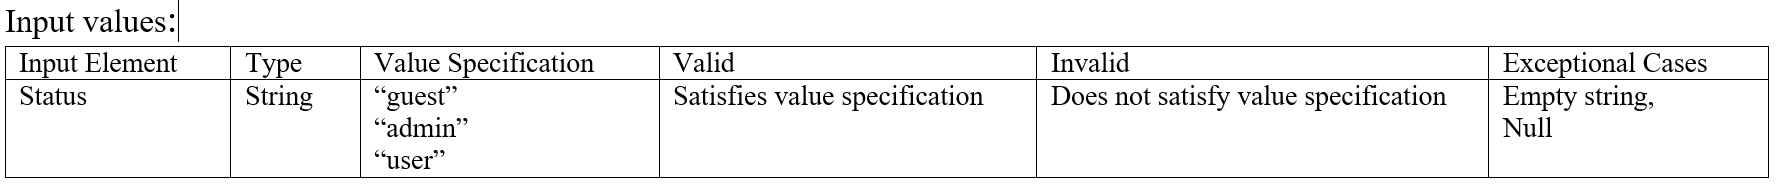
\includegraphics[width=180mm]{1.png}
\end{figure}
\begin{figure}[ht!]
\hspace*{-2.5cm} 
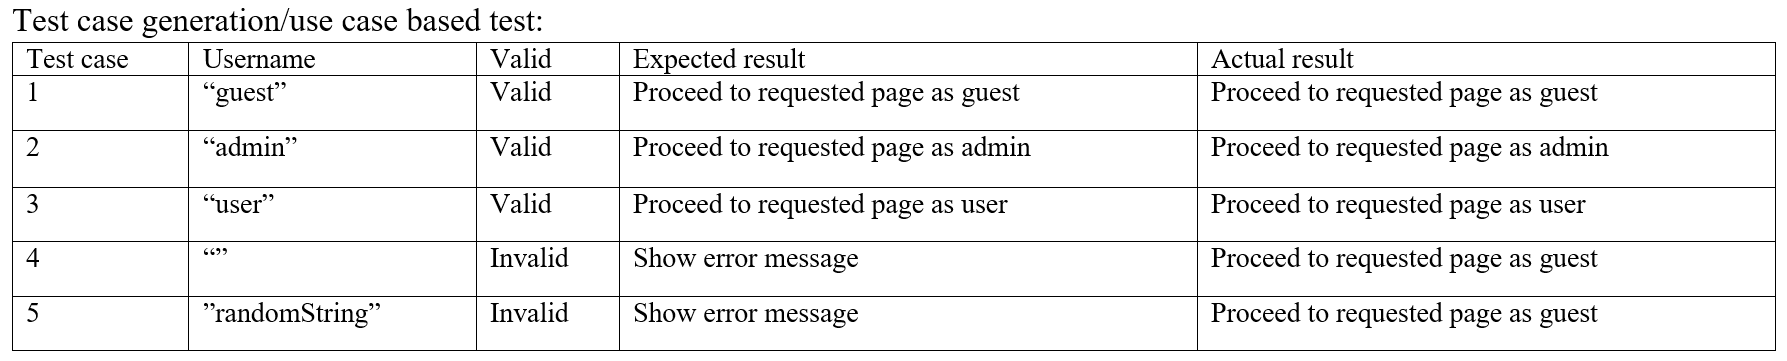
\includegraphics[width=180mm]{2.png}
\end{figure}
\subsection{Login}
\begin{figure}[H]
\hspace*{-2.5cm} 
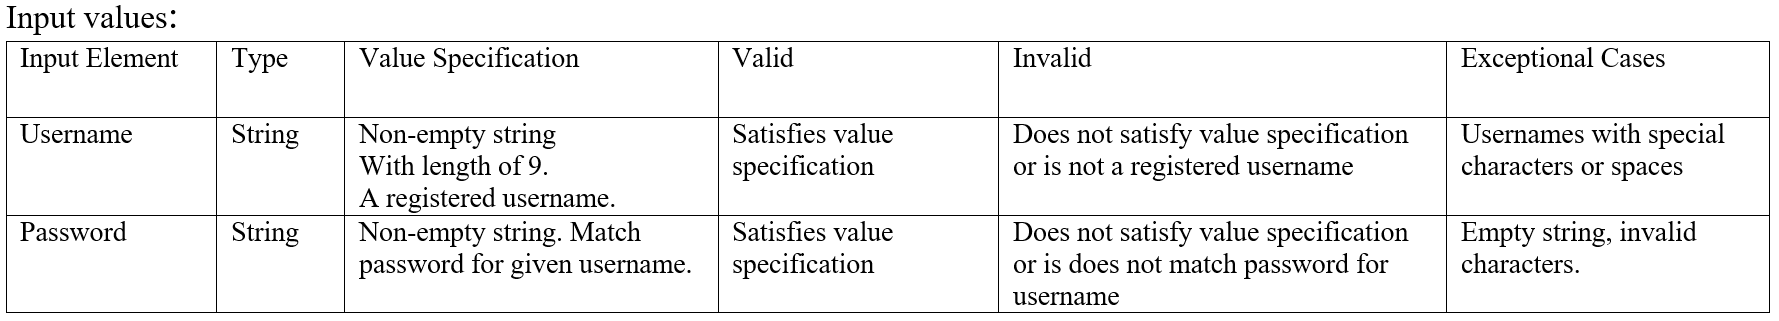
\includegraphics[width=180mm]{3.png}
\end{figure}
\begin{figure}[H]
\hspace*{-2.5cm} 
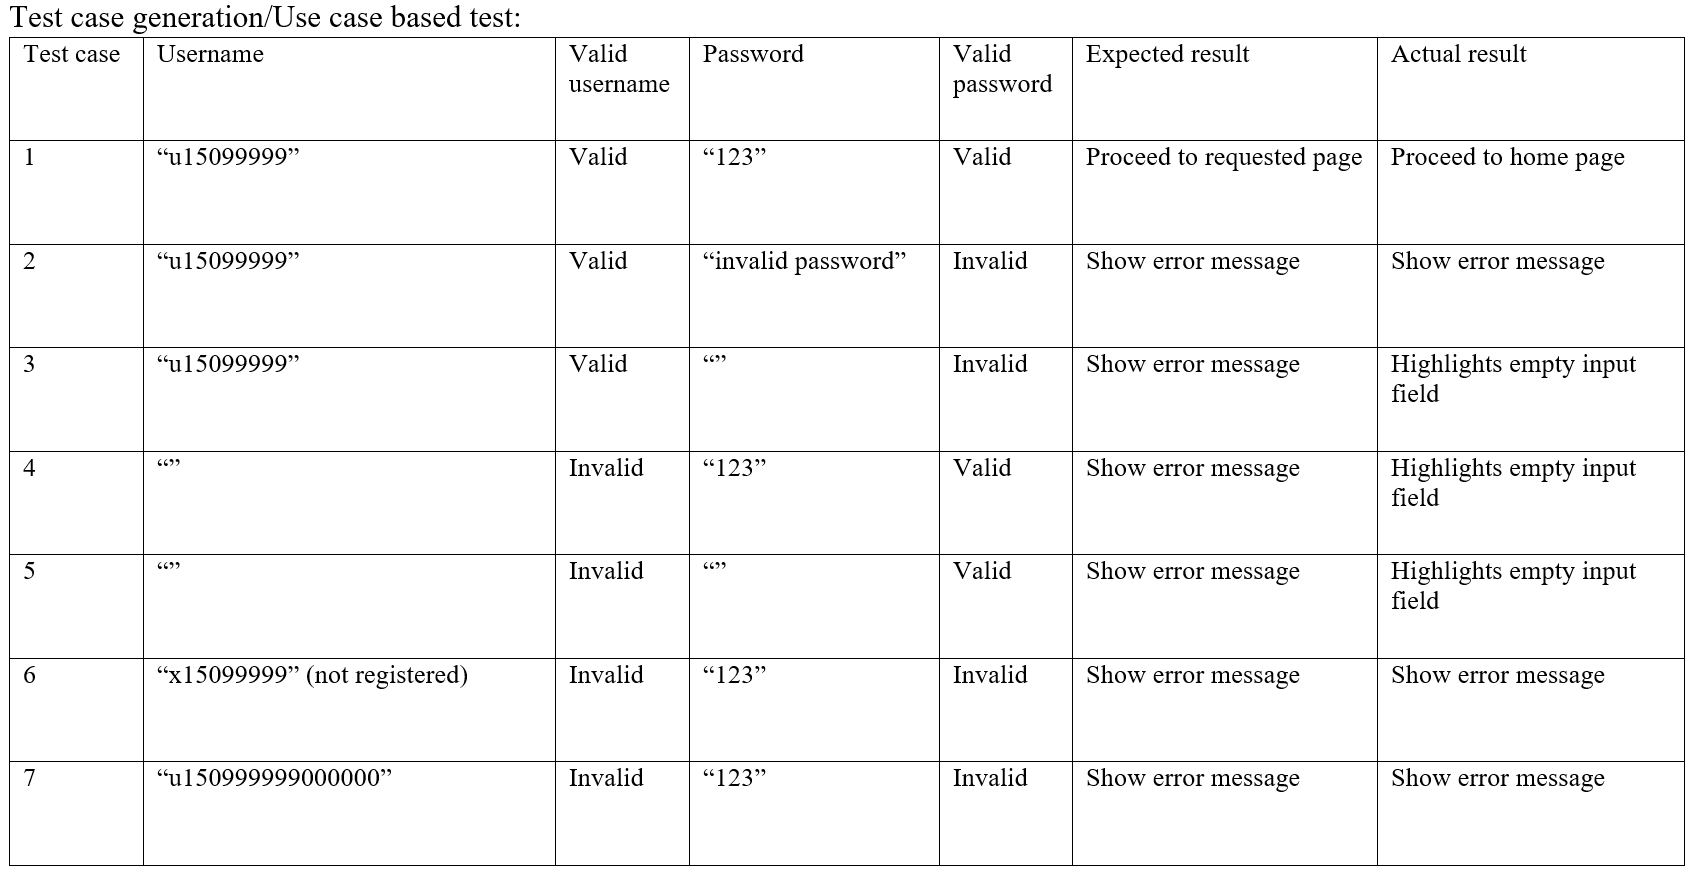
\includegraphics[width=180mm]{4.png}
\end{figure}
\subsection{Register}
\begin{figure}[H]
    \label{tab:example}
\hspace*{-2.5cm} 
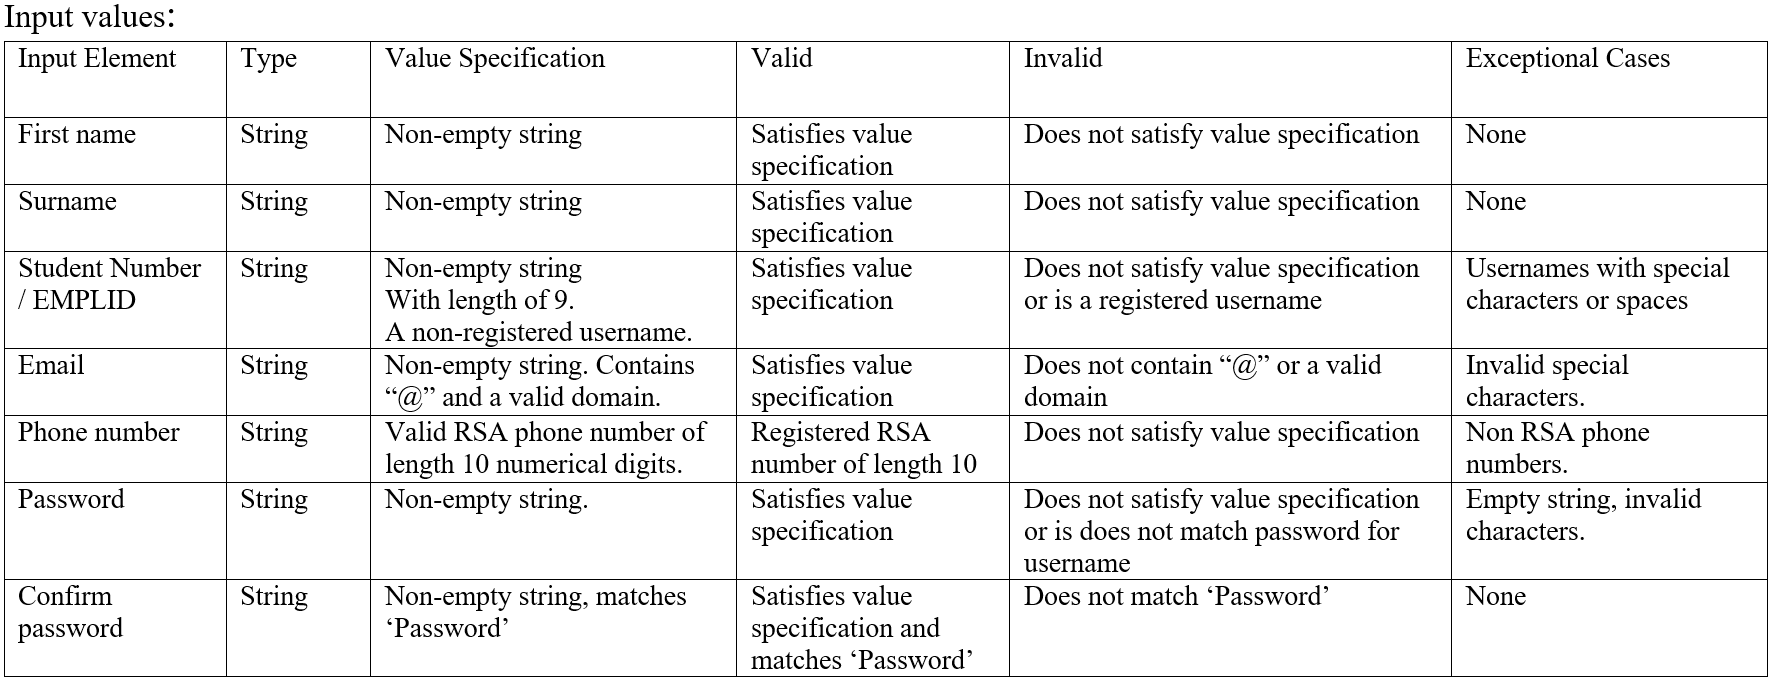
\includegraphics[width=180mm]{5.png}
\end{figure}
\begin{figure}[H]
\hspace*{-2.5cm} 
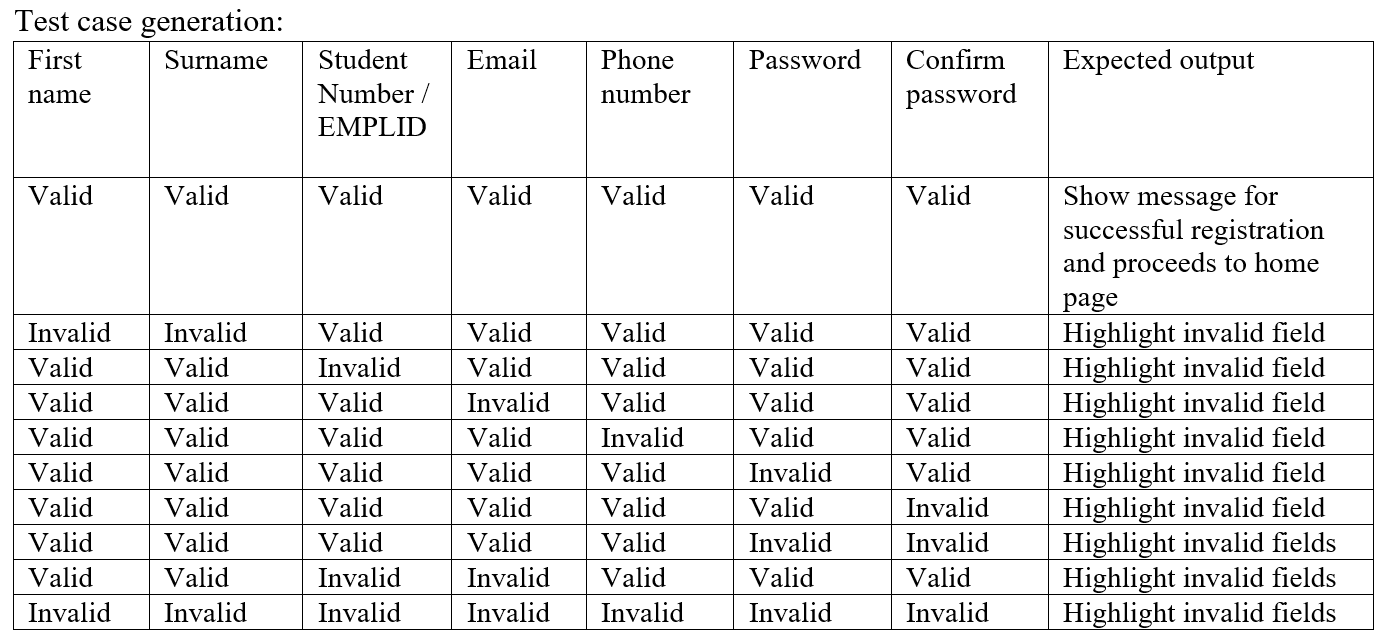
\includegraphics[width=180mm]{6.png}
\end{figure}
\begin{figure}[H]
\hspace*{-2.5cm} 
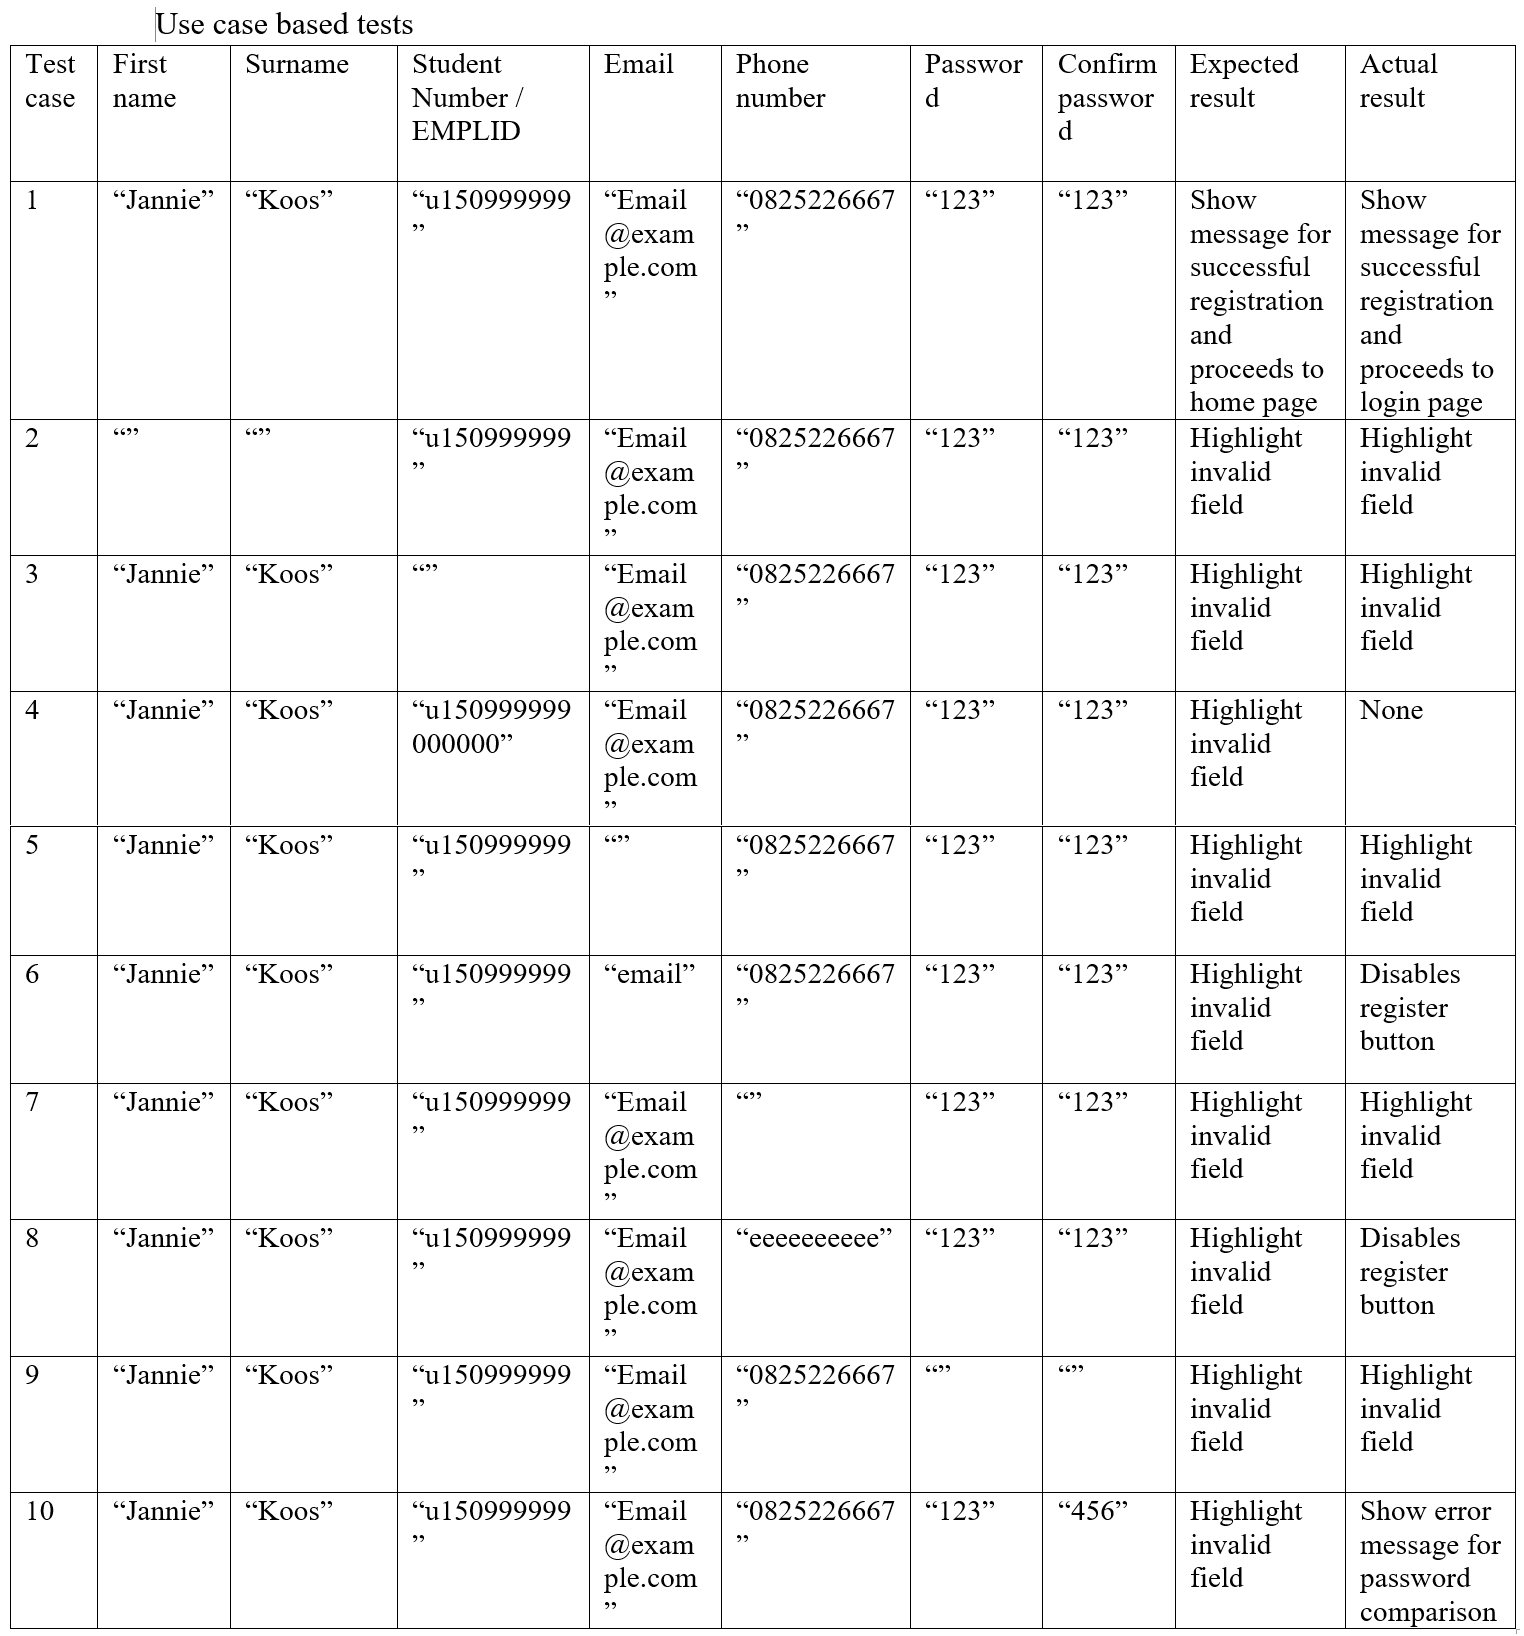
\includegraphics[width=180mm]{7.png}
\end{figure}
\subsection{View user profile}
\begin{figure}[ht!]
\hspace*{-2.5cm} 
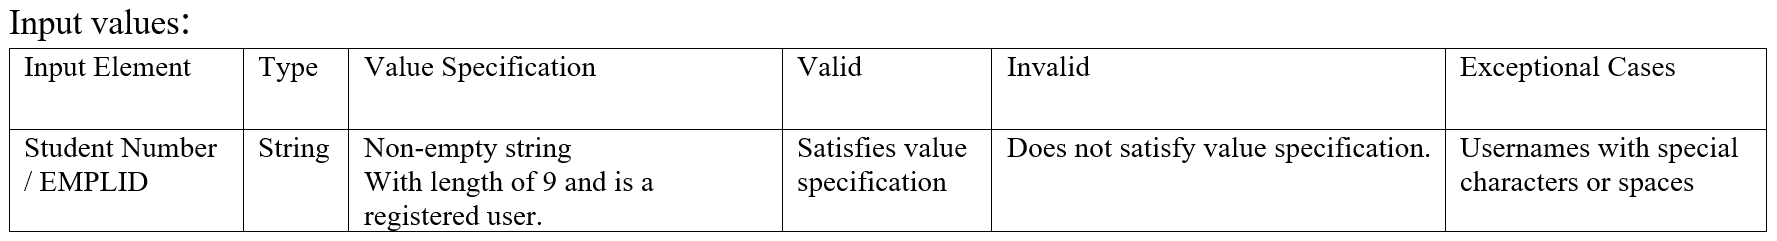
\includegraphics[width=180mm]{8.png}
\end{figure}
\begin{figure}[ht!]
\hspace*{-2.5cm} 
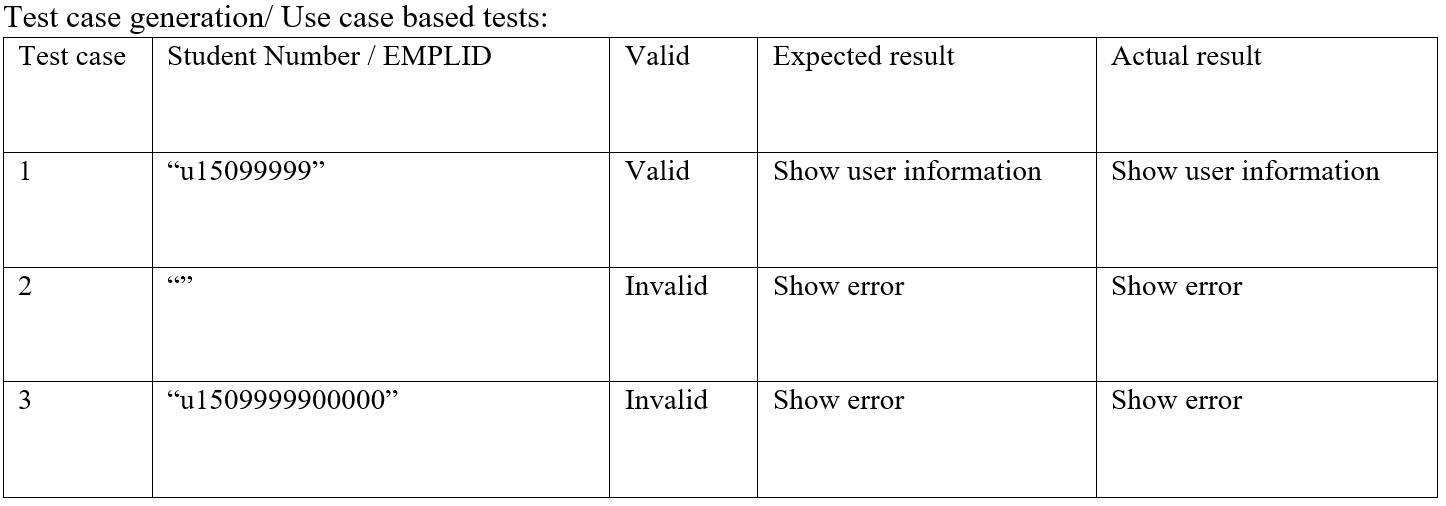
\includegraphics[width=180mm]{ViewTestCase.png}
\end{figure}
\subsection{Update user information}
\begin{figure}[H]
\hspace*{-2.5cm} 
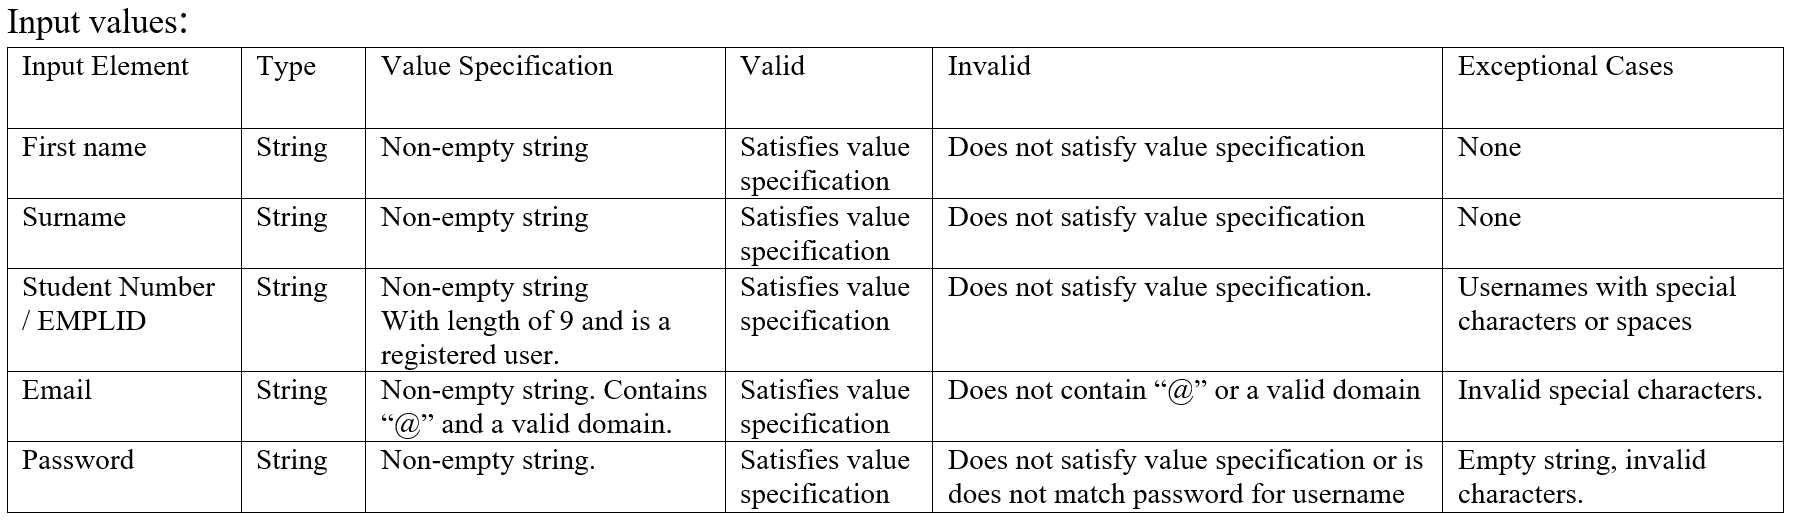
\includegraphics[width=180mm]{9.png}
\end{figure}
\begin{figure}[H]
\hspace*{-2.5cm} 
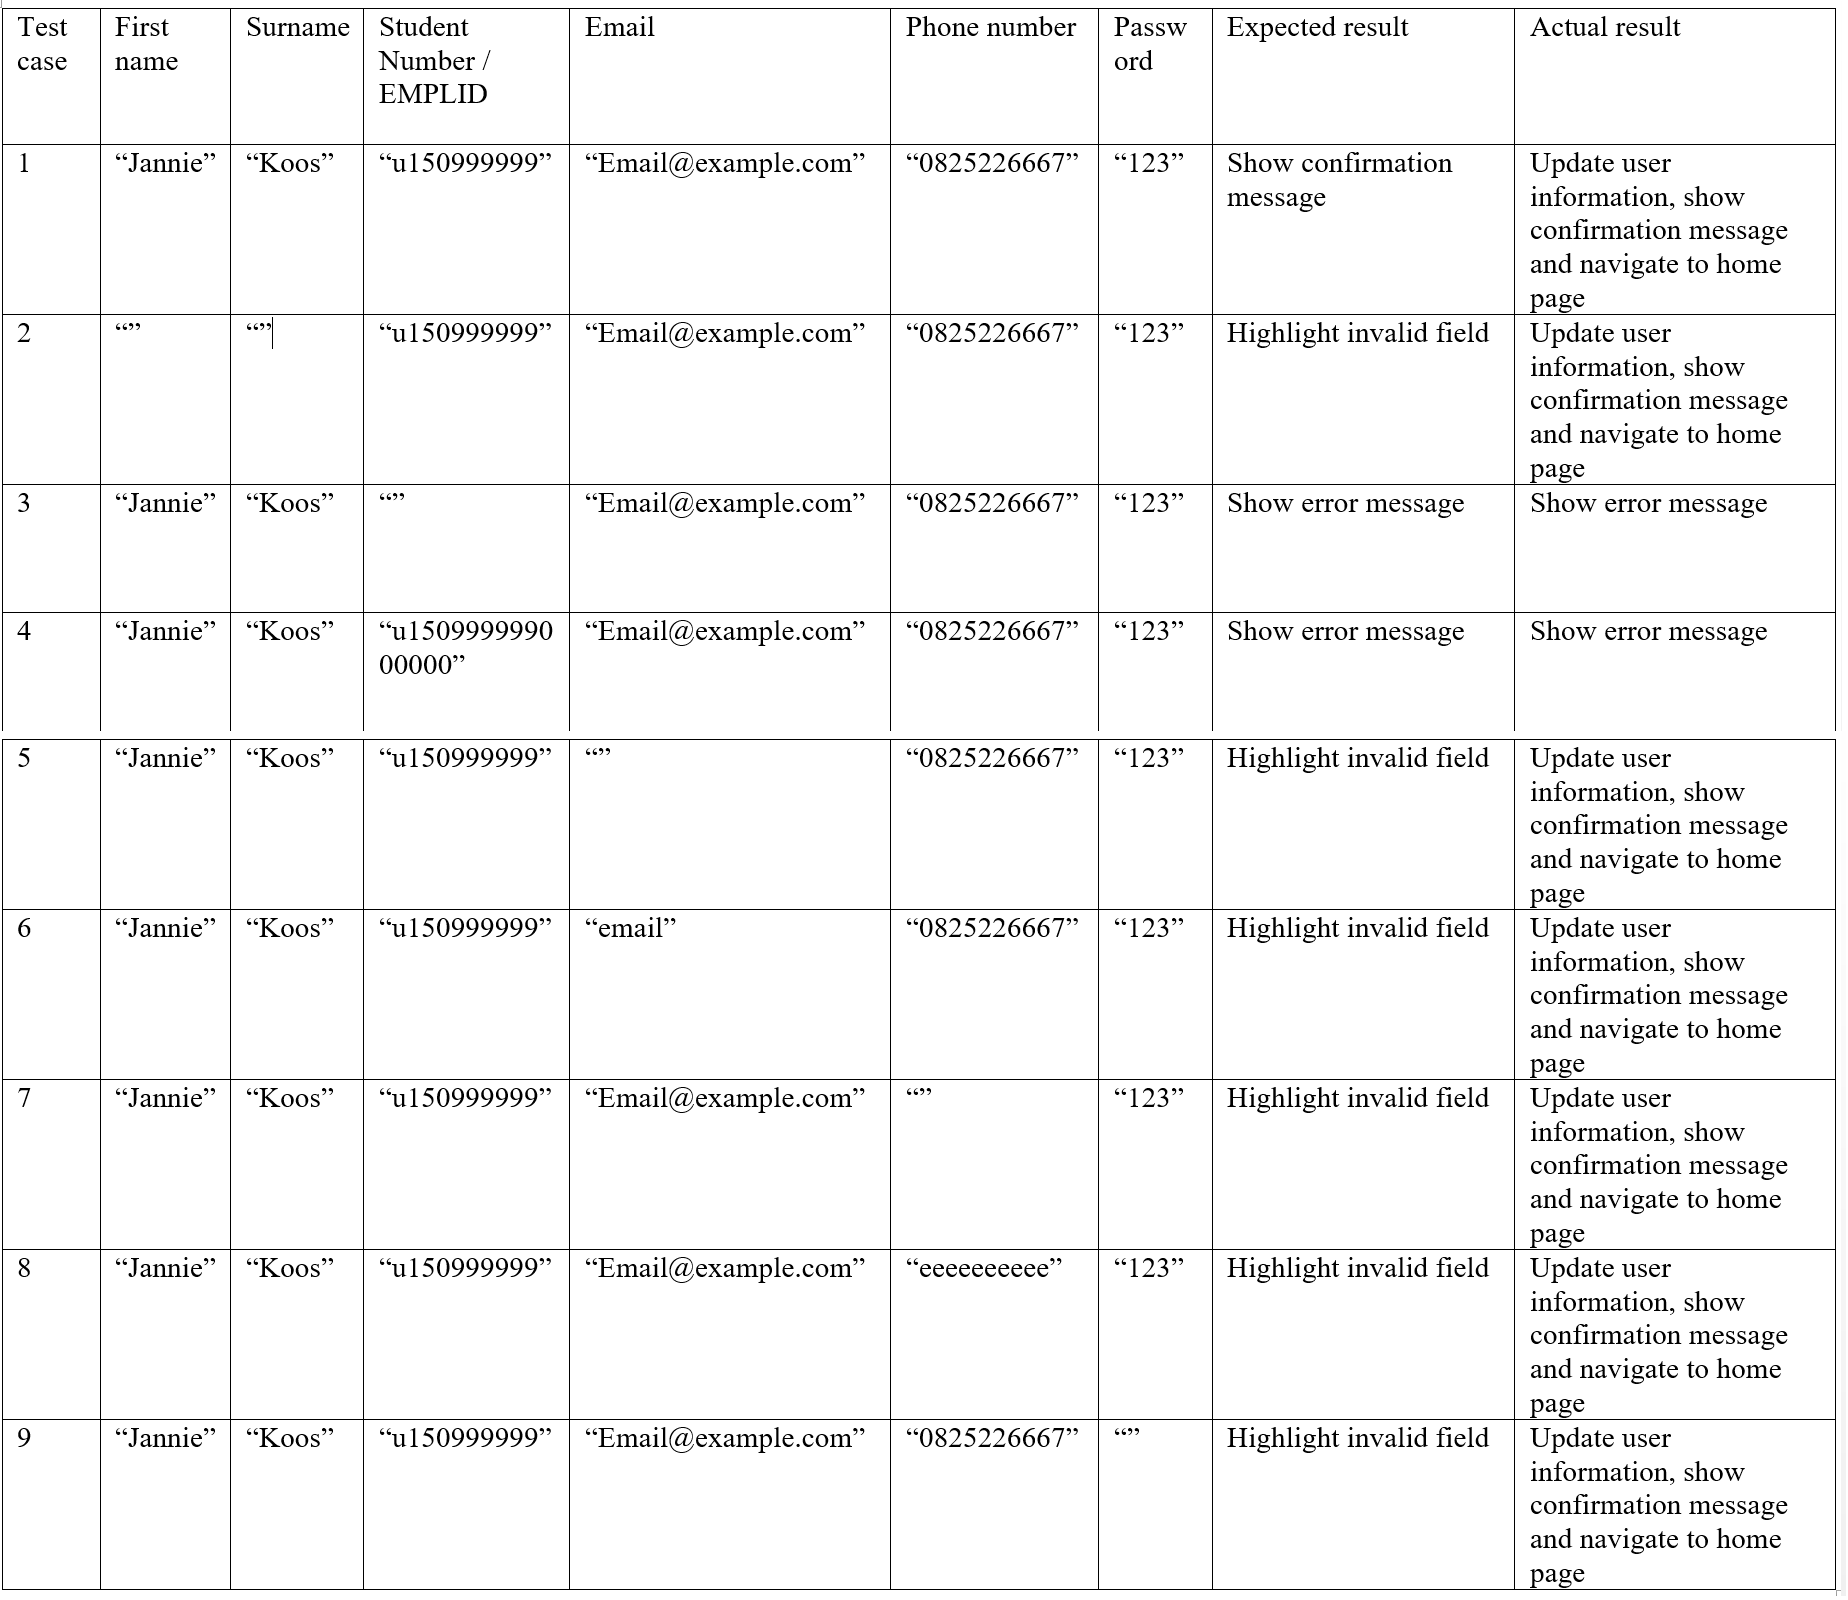
\includegraphics[width=180mm]{10.png}
\end{figure}
\begin{figure}[H]
\hspace*{-2.5cm} 
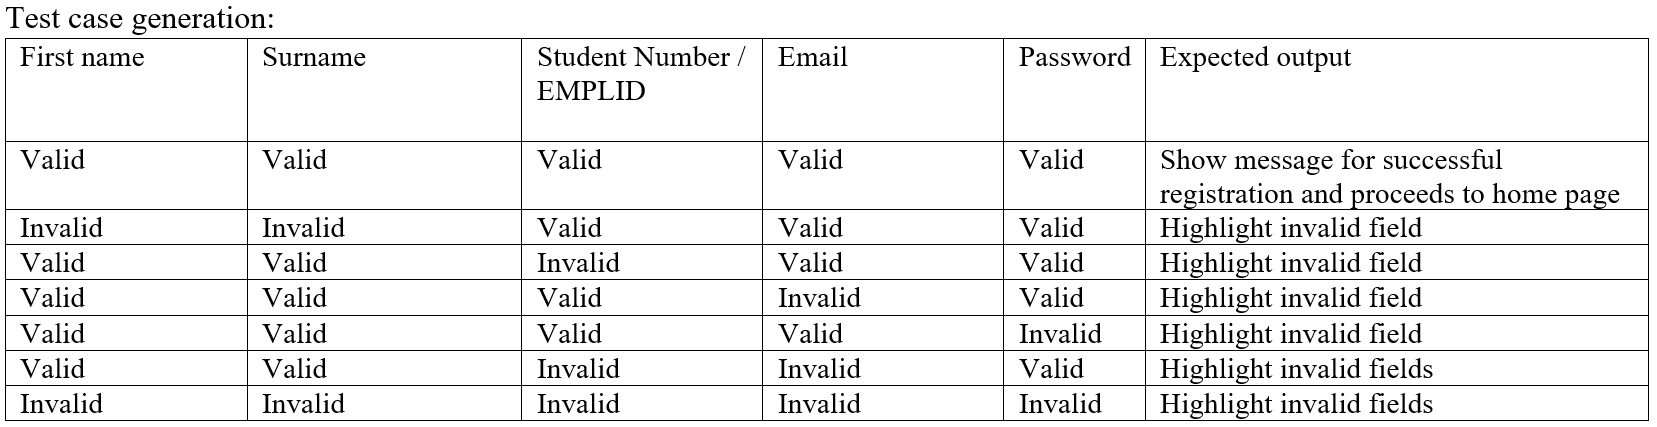
\includegraphics[width=180mm]{11.png}
\end{figure}
\subsection{Delete user profile}
\begin{figure}[ht!]
\hspace*{-2.5cm} 
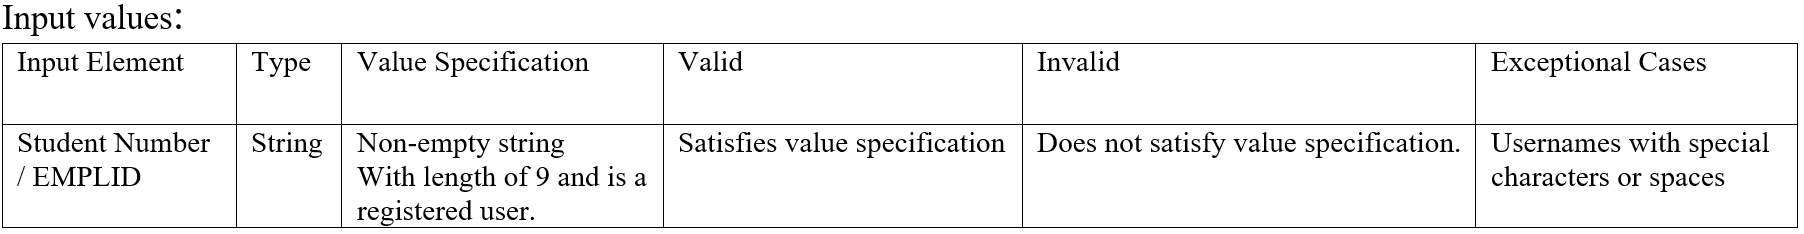
\includegraphics[width=180mm]{12.png}
\end{figure}
\begin{figure}[ht!]
\hspace*{-2.5cm} 
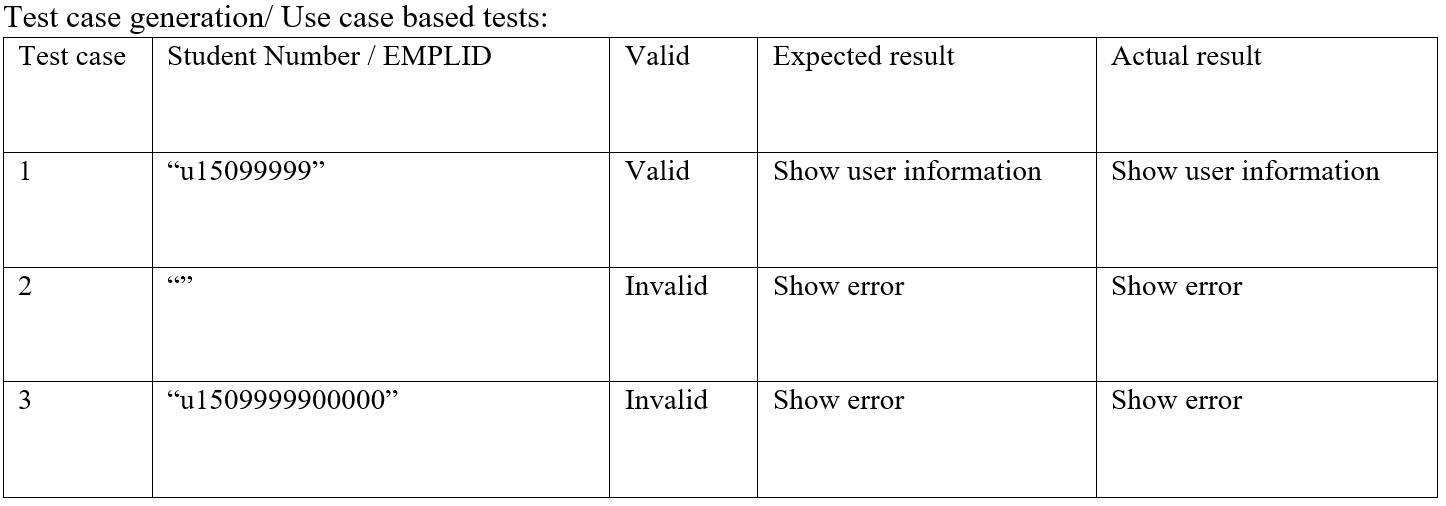
\includegraphics[width=180mm]{ViewTestCase.png}
\end{figure}
\clearpage
\subsection{Manage user information}
\begin{figure}[ht!]
\hspace*{-2.5cm} 
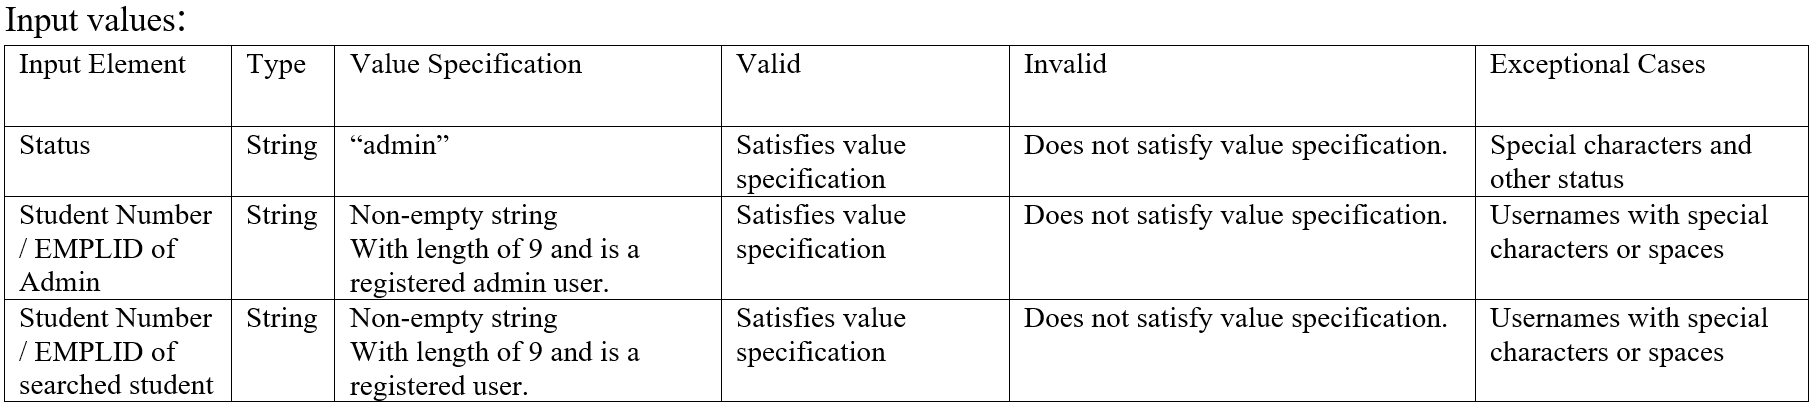
\includegraphics[width=180mm]{13.png}
\end{figure}
\begin{figure}[ht!]
\hspace*{-2.5cm} 
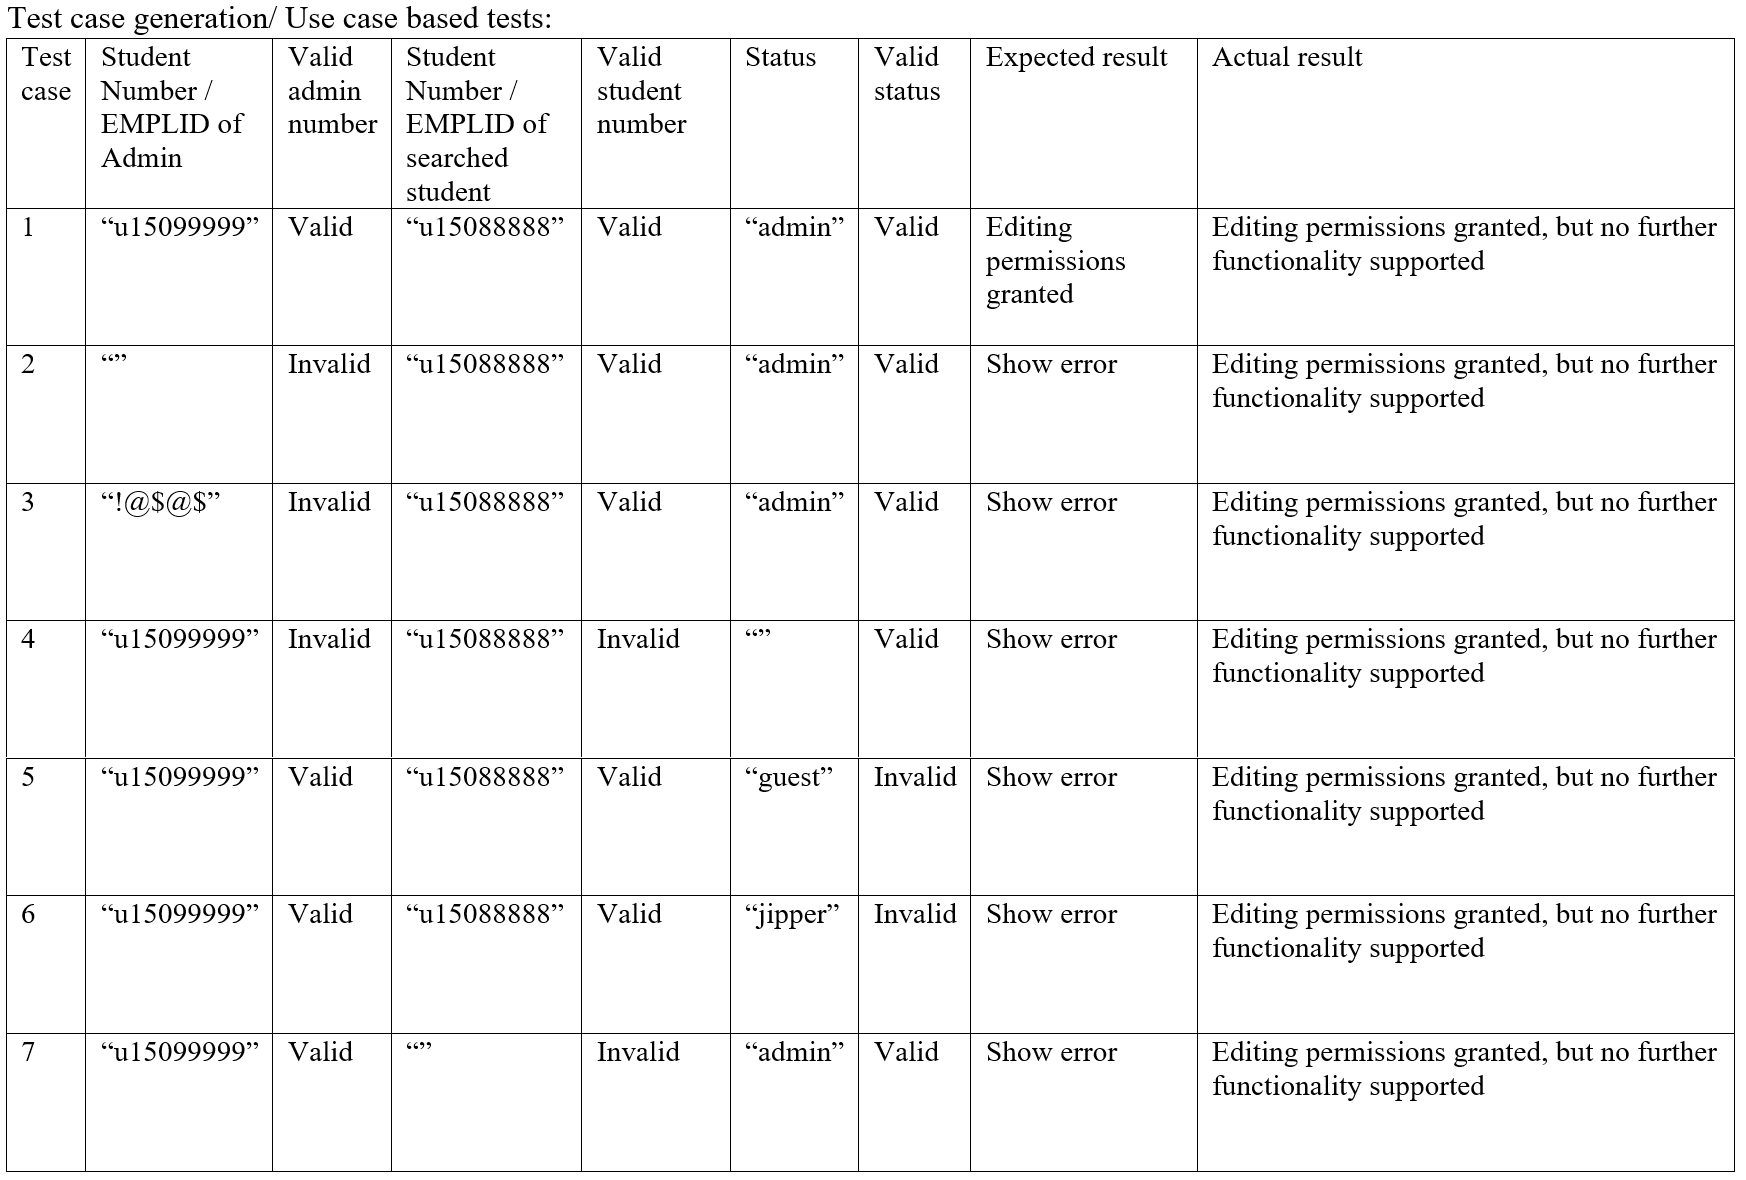
\includegraphics[width=180mm]{14.png}
\end{figure}
\clearpage
\begin{figure}[ht!]
\center
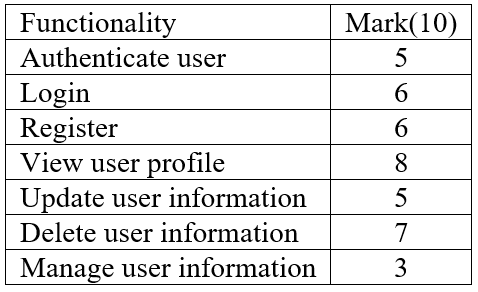
\includegraphics[width=60mm]{Marks.png}
\caption{Marks}
\end{figure}
\section{Non-functional requirements}
1.	Security\\
2.	User interface\\
3.	Performance\\
\subsection{Security}
\begin{itemize}
     \item It is possible to change your user privileges to admin by changing the status of the user in the URL to 'admin' at any page.\\
     Once changing status to admin the users can officially give admin rights to themselves and other users.
     \item Users can edit their user information to be empty strings especially for the password.\\
     A password is not required to change the password or any other user information.
     \item Users can login as other users by changing the user field in the URL to any valid user name.
   \end{itemize}
\subsection{User interface}
•	Features are hidden based on user status i.e. manage users tab is hidden to guest users, but is visible to admin users\\
\subsection{Performance}
\begin{figure}[H]
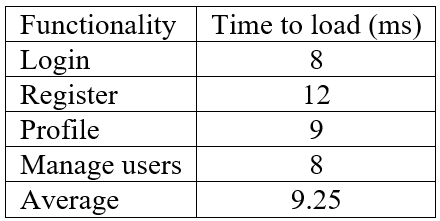
\includegraphics[width=60mm]{15.png}
\end{figure}
Performance-wise the pages were relatively fast and had nearly no noticeable loading time.
\section{Notifications}
\section{Service Contracts}
1.	Send Notification\\

\subsection{Send Notification}
\begin{figure}[H]
    \label{tab:example}
\hspace*{-2.5cm} 
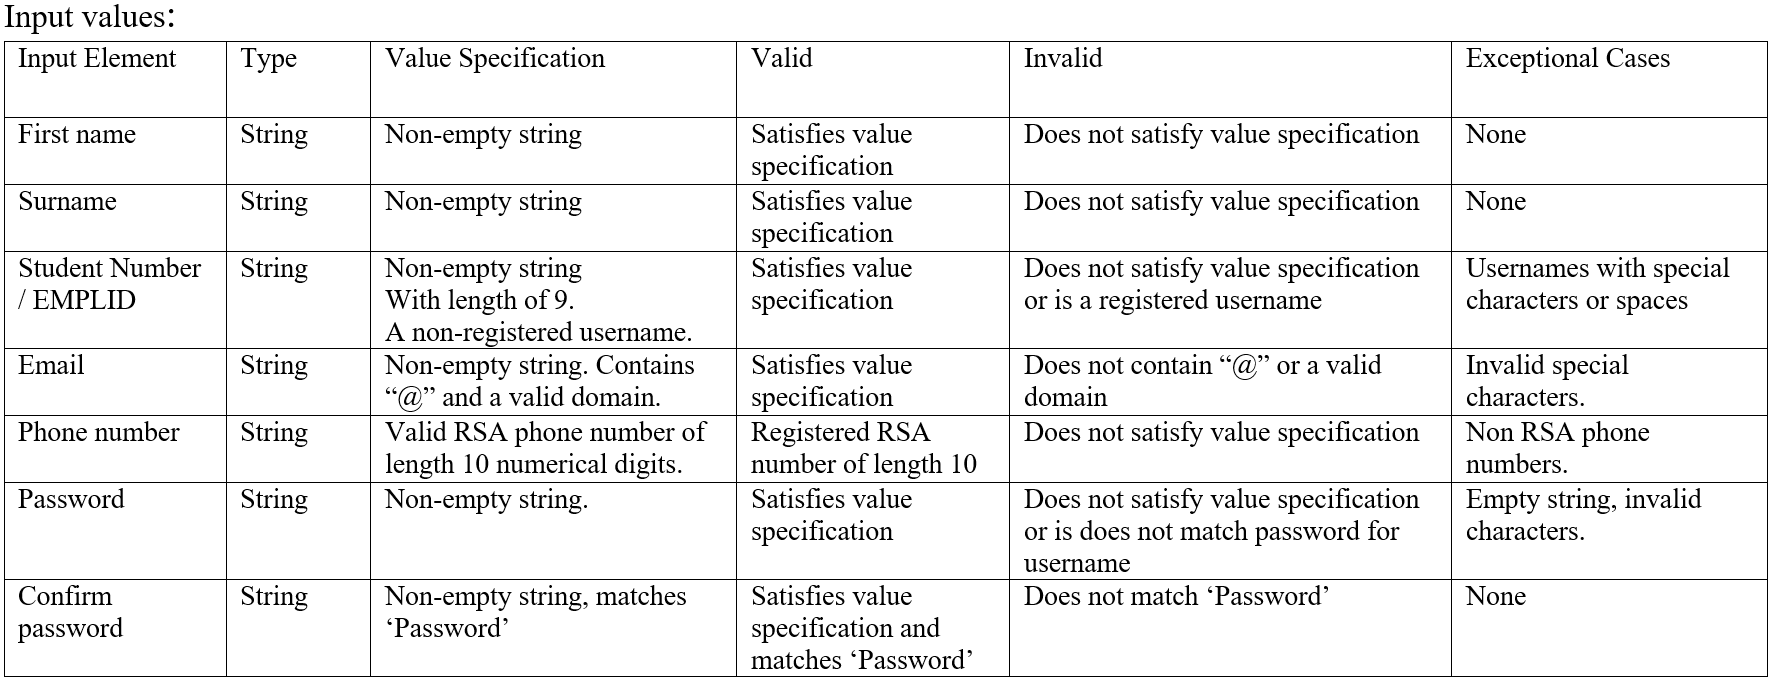
\includegraphics[width=180mm]{5.png}
\end{figure}

\begin{figure}[H]
\hspace*{-2.5cm} 
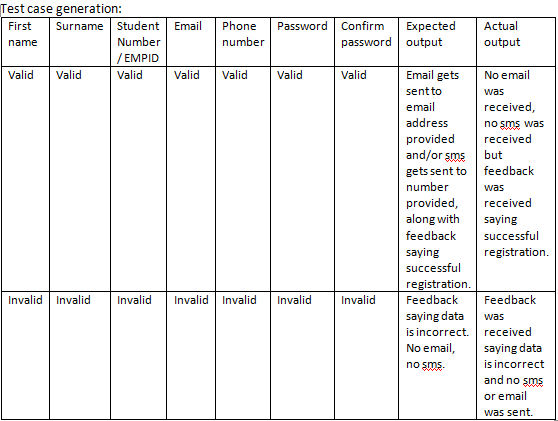
\includegraphics[width=180mm,height=90mm]{NotificationsTest.png}
\end{figure}

\section{Data}
\section{GIS}
\section{Service Contracts}
1.	Service GIS request\\
	a.	Get XYZ coordinates of a named location\\
2.	Add GIS information\\
	a.	Add a location with coordinates to the system\\
3.	Modify GIS information\\
4.	Remove GIS information\\
5.	Update GIS Map\\
6.	Modify GIS Map\\
\subsection{Service GIS request}
\begin{figure}[ht!]
\hspace*{-2.5cm} 
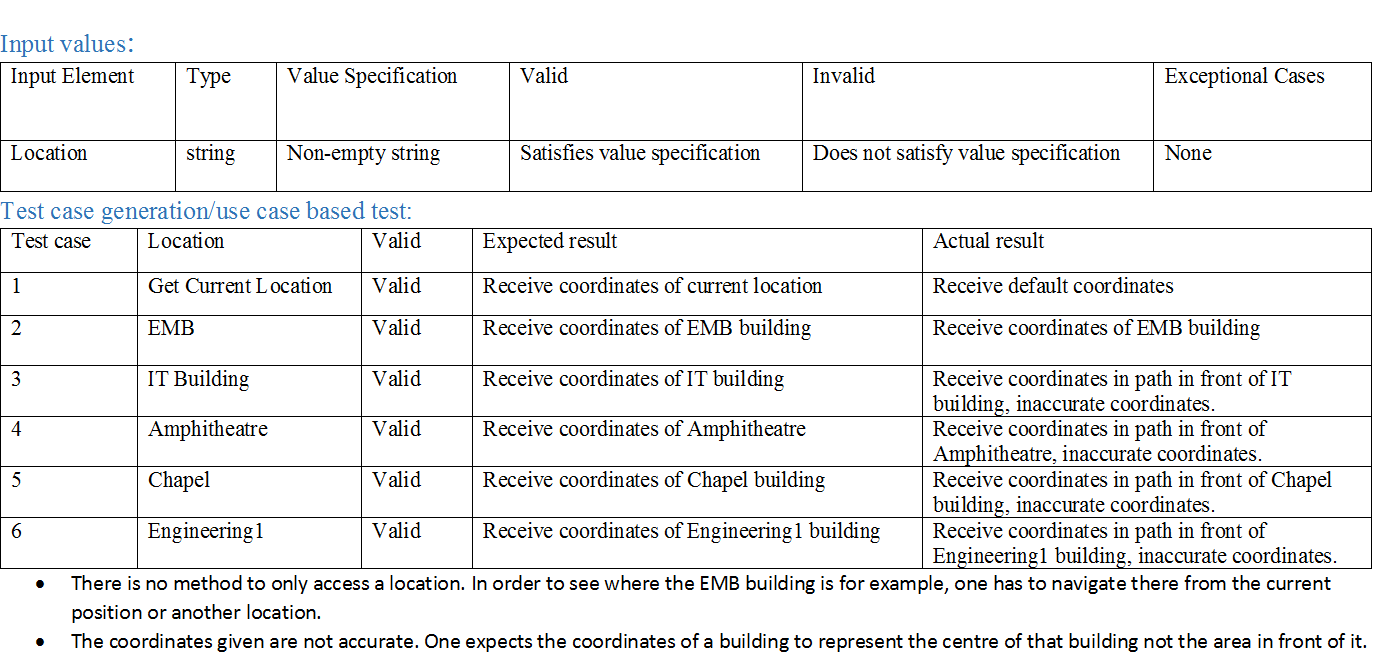
\includegraphics[width=180mm]{ServiceGISReq.png}
\end{figure}
\subsection{Add GIS information}
\begin{figure}[ht!]
\hspace*{-2.5cm} 
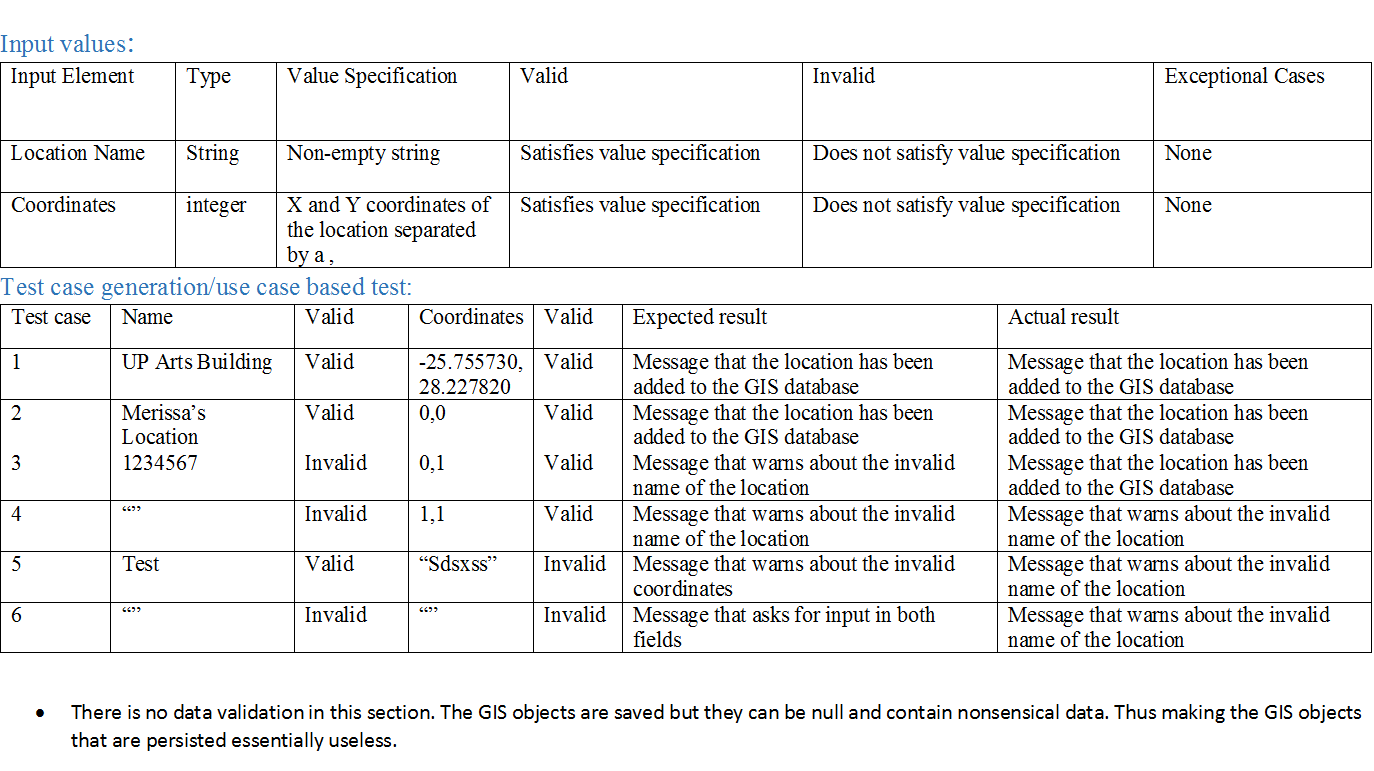
\includegraphics[width=180mm]{AddGISInformation.png}
\end{figure}
\subsection{Modify GIS information}
\begin{figure}[H]
\label{tab:example}
\hspace*{-2.5cm} 
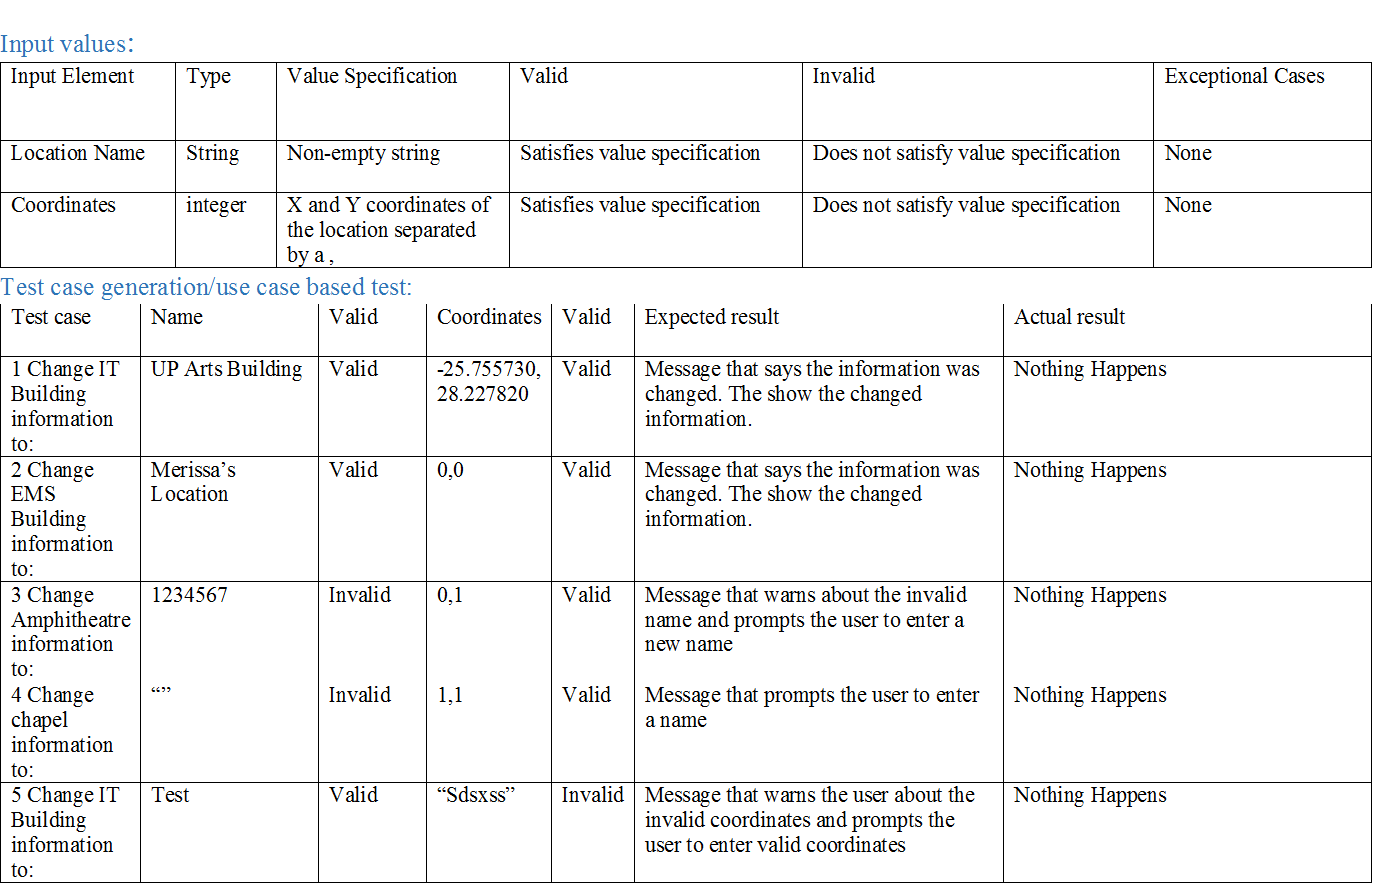
\includegraphics[width=180mm]{ModifyGISInformation.png}
\end{figure}
\subsection{Remove GIS information}
\begin{figure}[ht!]
\hspace*{-2.5cm} 
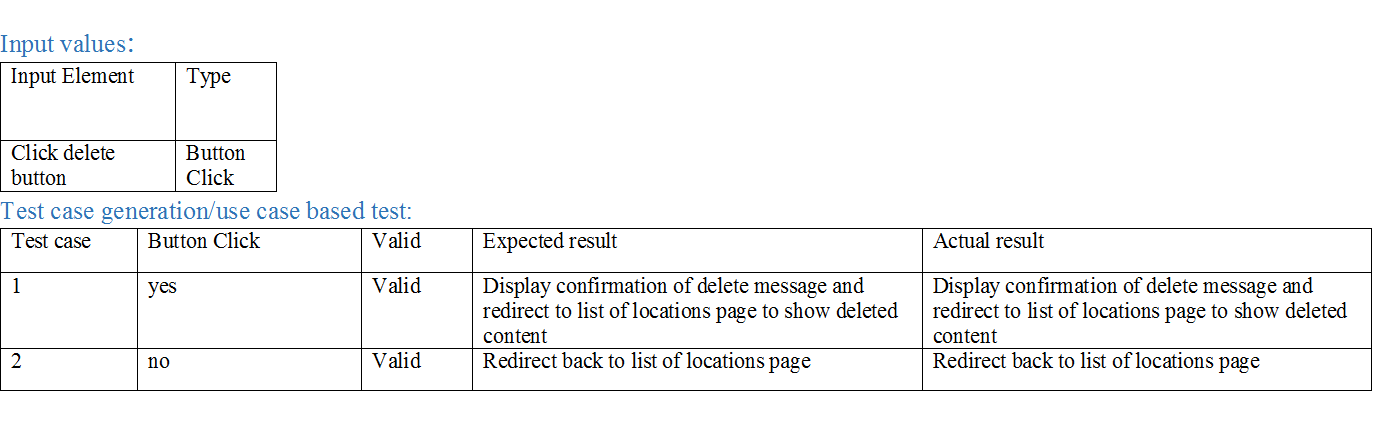
\includegraphics[width=180mm]{DeleteGISInformation.png}
\end{figure}
\subsection{Update GIS Map}
\begin{figure}[H]
\hspace*{-2.5cm} 
\includegraphics[width=180mm]{UpdateGISMap.png}
\end{figure}
\subsection{Modify GIS Map}
There is no functionality to modify the given map.
\section{Non-functional requirements}
\begin{figure}[H]
\hspace*{-2.5cm} 
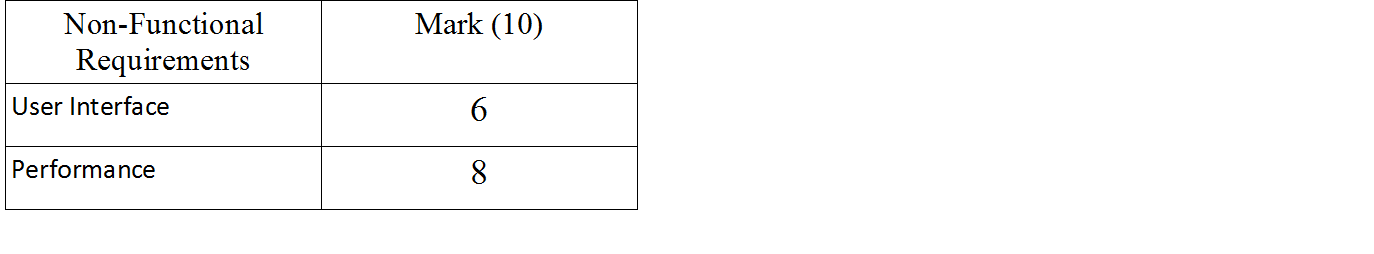
\includegraphics[width=180mm]{NFRMarks.png}
\end{figure}
\subsection{User interface}
•	The interface for adding GIS information is confusing. After saving the required information into the database, the information stays open and you cannot enter a new object until you refresh the page.
•	There is no limit on how far the user can zoom in and out. This leaves the user fully able to see the entire world map and view other locations, which should not be able to happen in the NavUp application.
•	The map can be dragged outside the boundaries of campus. This is not in the scope of the application.
•	The interface for GIS data modification is confusing. The labels do not guide the user in what he or she is doing in any way. 
\section{Points of interest}
\section{Navigation}
\end{document}
